% Options for packages loaded elsewhere
\PassOptionsToPackage{unicode}{hyperref}
\PassOptionsToPackage{hyphens}{url}
%
\documentclass[
  12,
]{paper}
\usepackage{lmodern}
\usepackage{amssymb,amsmath}
\usepackage{ifxetex,ifluatex}
\ifnum 0\ifxetex 1\fi\ifluatex 1\fi=0 % if pdftex
  \usepackage[T1]{fontenc}
  \usepackage[utf8]{inputenc}
  \usepackage{textcomp} % provide euro and other symbols
\else % if luatex or xetex
  \usepackage{unicode-math}
  \defaultfontfeatures{Scale=MatchLowercase}
  \defaultfontfeatures[\rmfamily]{Ligatures=TeX,Scale=1}
\fi
% Use upquote if available, for straight quotes in verbatim environments
\IfFileExists{upquote.sty}{\usepackage{upquote}}{}
\IfFileExists{microtype.sty}{% use microtype if available
  \usepackage[]{microtype}
  \UseMicrotypeSet[protrusion]{basicmath} % disable protrusion for tt fonts
}{}
\makeatletter
\@ifundefined{KOMAClassName}{% if non-KOMA class
  \IfFileExists{parskip.sty}{%
    \usepackage{parskip}
  }{% else
    \setlength{\parindent}{0pt}
    \setlength{\parskip}{6pt plus 2pt minus 1pt}}
}{% if KOMA class
  \KOMAoptions{parskip=half}}
\makeatother
\usepackage{xcolor}
\IfFileExists{xurl.sty}{\usepackage{xurl}}{} % add URL line breaks if available
\IfFileExists{bookmark.sty}{\usepackage{bookmark}}{\usepackage{hyperref}}
\hypersetup{
  pdftitle={Intra-Party Affect},
  pdfauthor={Rob Lytle},
  hidelinks,
  pdfcreator={LaTeX via pandoc}}
\urlstyle{same} % disable monospaced font for URLs
\usepackage{graphicx}
\makeatletter
\def\maxwidth{\ifdim\Gin@nat@width>\linewidth\linewidth\else\Gin@nat@width\fi}
\def\maxheight{\ifdim\Gin@nat@height>\textheight\textheight\else\Gin@nat@height\fi}
\makeatother
% Scale images if necessary, so that they will not overflow the page
% margins by default, and it is still possible to overwrite the defaults
% using explicit options in \includegraphics[width, height, ...]{}
\setkeys{Gin}{width=\maxwidth,height=\maxheight,keepaspectratio}
% Set default figure placement to htbp
\makeatletter
\def\fps@figure{htbp}
\makeatother
\setlength{\emergencystretch}{3em} % prevent overfull lines
\providecommand{\tightlist}{%
  \setlength{\itemsep}{0pt}\setlength{\parskip}{0pt}}
\setcounter{secnumdepth}{-\maxdimen} % remove section numbering
\usepackage[margin=1in]{geometry}
\usepackage{caption}
\usepackage{amsmath}
\usepackage{mathrsfs}
\usepackage{float}
\usepackage{natbib}
\bibliographystyle{apsr}
\usepackage{graphicx}
\graphicspath{ {../fig/} }
\usepackage{setspace}
\usepackage[super]{nth}
\usepackage{booktabs}
\usepackage{makecell}
\usepackage{amsmath}
\usepackage{dcolumn}
\usepackage{hyperref}
\usepackage{booktabs}
\usepackage{longtable}
\usepackage{array}
\usepackage{multirow}
\usepackage{wrapfig}
\usepackage{float}
\usepackage{colortbl}
\usepackage{pdflscape}
\usepackage{tabu}
\usepackage{threeparttable}
\usepackage{threeparttablex}
\usepackage[normalem]{ulem}
\usepackage{makecell}
\newlength{\cslhangindent}
\setlength{\cslhangindent}{1.5em}
\newenvironment{cslreferences}%
  {\setlength{\parindent}{0pt}%
  \everypar{\setlength{\hangindent}{\cslhangindent}}\ignorespaces}%
  {\par}

\title{Intra-Party Affect}
\author{Rob Lytle}
\date{}

\begin{document}
\maketitle

\doublespacing

In 2008, despite her roll as Democratic standard-bearer, Supporters of
Hillary Clinton's primary campaign were colder towards their party than
any other group of Democratic primary voters on the ANES 100-point
Feeling Thermometer. Clinton's defeat by Barack Obama in June of 2008
spawned the ``Party Unity My Ass'' movement, engaging in various forms
of protest against the DNC and pledging \emph{en masse} not to support
the (relative) party outsider Barack Obama in the general
election\footnote{\url{https://www.washingtonpost.com/wp-dyn/content/article/2008/06/26/AR2008062604162.html?tid=a_inl_manual}}.

Clinton supporters' posture towards their party in 2016 bore little
semblance to that of the '08 race. Bernie Sanders---a former independent
and self-identified socialist---leaned into the role of an insurgent,
anti-establishment candidate; predicating his campaign on a conflict
between the working-class and the elites of both major parties. Sanders
supporters, angry with the DNC and reluctant to support Clinton in
November led a loosely organized movement of Democratic party
discontents to found groups like \emph{Justice Democrats} and expand
membership of organizations like the \emph{Democratic Socialists of
America} and various state and local progressive caucuses to protest
perceived slights by the party establishment and support further left
and anti-establishment down-ballot candidates.

This is not particularly surprising on its own. Sanders campaigned
against the party establishment---it is not a stretch that he would
attract those disillusioned or unhappy with the party. The story is more
complicated. Republican supporters of Donald Trump---whose campaign was
even more exuberantly hostile towards the Republican party---were
\emph{warmer} towards their party than any other candidates' supporters,
despite the mutual hostility between Trump and established Republican
elites.

In the last decade, factions like the Tea Party and alt-right in the
Republican Party and Progressives and Democratic Socialists in the
Democratic party have presented challenges to their party's status-quo.
While factions like the ``Blue Dog Democrats'' or ``Main Street
Republicans'' are nothing new and have long communicated a brand
\emph{separate} from their party (Clarke 2017), the brand being
communicated has not necessarily been hostile to mainline party elites.
The same cannot be said for more recently ascendant groups like the
Justice Democrats, Tea Party, or alt-right. Candidates aligned with
these factions often explicitly position themselves as adversarial to
established, mainstream members of their party, challenging
``establishment'' representatives in primary battles and expressing
dissatisfaction with---or open hostility towards---party leaders. These
contests occasionally garner national attention, as was the case with
Democrats Alexandria Ocasio Cortez's and Marie Newman's---both Justice
Democrats---successful challenges of Joe Crowley and Dan Lipinski
respectively. During the Obama administration, slew of Tea Party
affiliated candidates including Ted Cruz and Rand Paul achieved national
prominence after winning crowded primaries with the anti-establishment
branding of the Tea Party. More recently, at least 81 candidates
supporting the Q-Anon conspiracy theory have won primaries in House and
Senate races, 24 of whom will be on the ballot in
November\footnote{https://www.mediamatters.org/qanon-conspiracy-theory/here-are-qanon-supporters-running-congress-2020}.
One of these candidates, Marjorie Taylor Greene, resides in a deep-red
district and is almost certain to take office in January.

There is evidence that the divisions between elite co-partisans are
meaningful at the mass level. Using the case 2016 Democratic primary
(Wronski et al. 2018) demonstrate that Democrats in 2016 primary were
divided along authoritarian lines. Primary voters scoring high in
authoritarian personality traits were more likely to support Hillary
Clinton---those with few authoritarian tendencies were likely to be
supporters of Bernie Sanders. {[}add more to this section, further build
theory of why party loss matters{]}

Across this backdrop of salient intra-party division not only has warmth
towards the out-party declined {[}Iyengar, Sood, and Lelkes (2012);
iyengar2018strengthening{]} but---particularly for Republicans---in
party warmth as well Klar, Krupnikov, and Ryan (2018). What has been
described as affective polarization may be better characterized as a
generalized decline in warmth towards the political system. As in-party
affect declines, so too has the role of positive partisanship
(attachment to one's own party) been supplanted by hostility towards the
out-party as a predictor of voting behavior (Iyengar and Krupenkin
2018). \textbf{An increasing number of Democrats and Republicans, voters
and nonvoters, and partisans and non-partisans are lukewarm or
cold---not just towards an out-party but towards both major parties}.
With this research note, I describe in detail how the distribution of
mass-level partisan affect has shifted to provide context for the above
findings. I close by discussing the implications of this shift and
suggest avenues for future research.

\hypertarget{results}{%
\section{Results}\label{results}}

\hypertarget{trends-in-intra-party-affect}{%
\subsection{Trends in Intra-Party
Affect}\label{trends-in-intra-party-affect}}

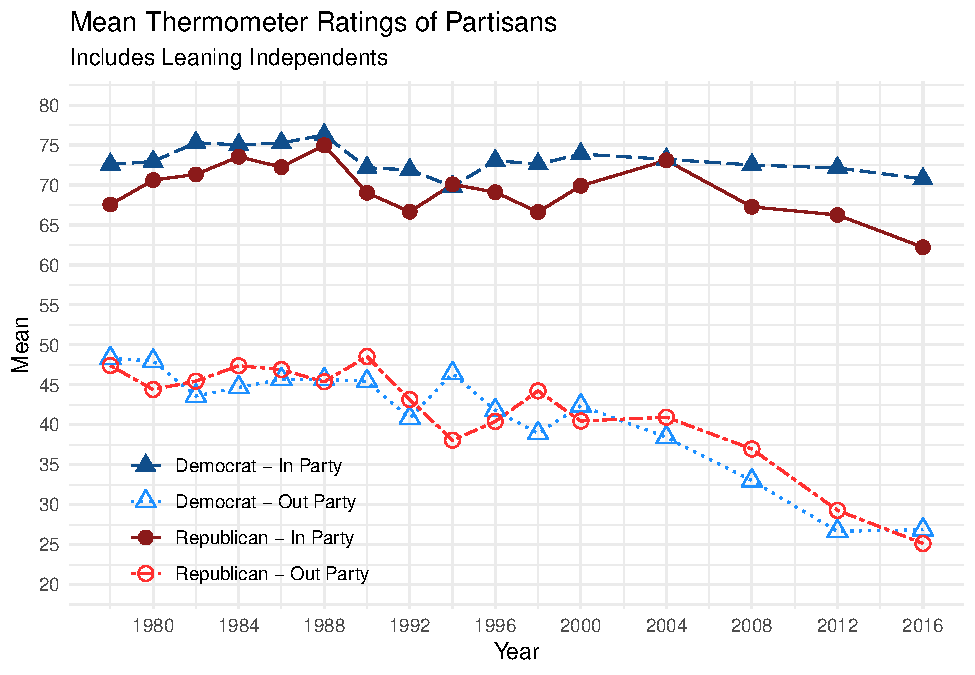
\includegraphics{intra-party-note_files/figure-latex/unnamed-chunk-2-1.pdf}

\emph{\textbf{Fig 1:} Mean in-party ANES feeling thermometers have
experienced a modest decline.}

As shown in Figure 1, mean out party feeling thermometers for Democrats
and Republicans have obviously declined. We also a see a decline in
Republican's in party FTs since 2004, and only a slight decline in those
of Democrats. Partisans remain much warmer (on average) towards their
party than the opposition this---particularly in the case of
Republicans---is in spite of a decline in average in-party FTs.

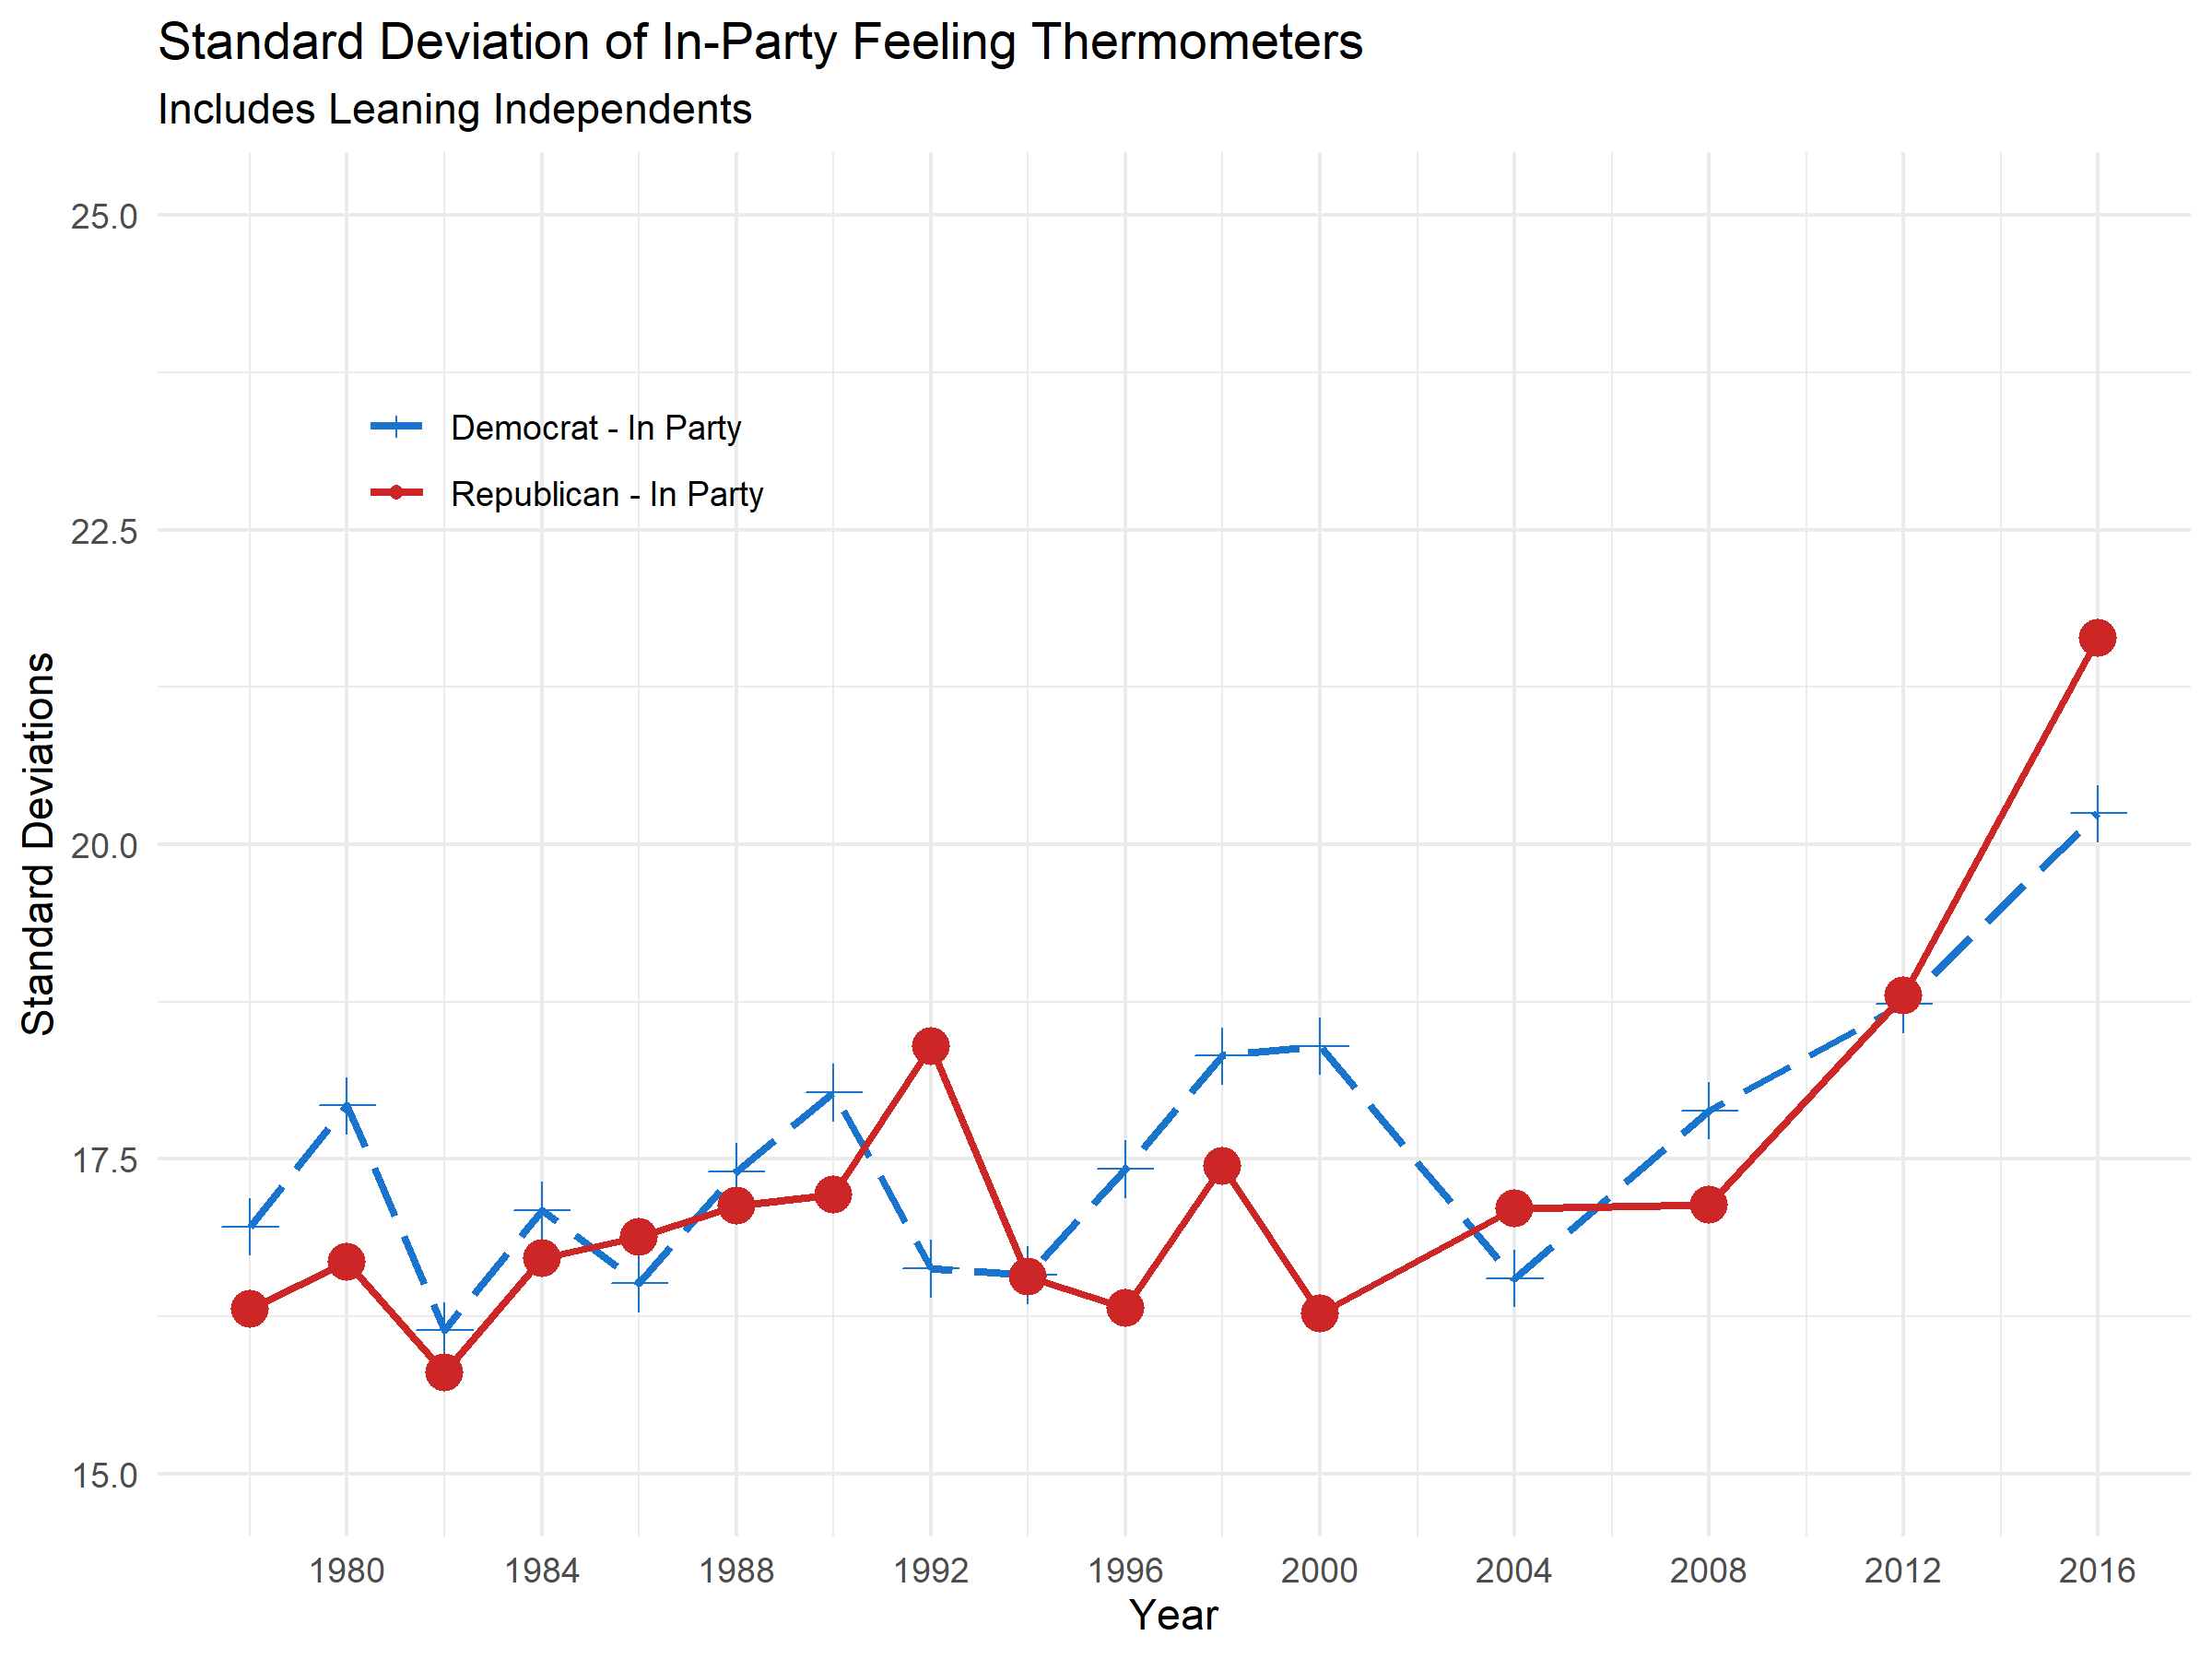
\includegraphics{fig/gg-sd-ns.png} \emph{\textbf{Fig 2:} The variance
within in-party feeling thermometers has increased since 2004.}

From 2004--2016 the variation within in-party feeling thermometer
ratings has increased. the standard deviation of Republicans' in-party
FTs increased from about 17--21 in this period, while Democrats'
increased from 16-20. While the magnitude of this increase does not
sound particularly impressive, \emph{Fig. 2} makes clear that a period
of increasing affective heterogeneity as large or prolonged as this has
not been observed at any other point over the range of ANES data.

As variance increases, so to has the proportion of partisans who rate
their own party below a 50---a substantively meaningful threshold
indicating that partisans are more cold than warm toward their own
party. When leaning independents are included---following (Klar and
Krupnikov 2016) ---10\% of Democrats and almost 20\% of Republicans are
found to be cold towards their own party (up from 5\% each in 2004),
while a sample which excludes leaning independents indicates 13\% of
Republicans and 8\% of Democrats to be cold. Regardless of the cut-off
point used to indicate cold affect, or the strength of partisans'
identification with their party, the trend is robust---more partisans
were cold to their party than has been observed at any point across the
available data.

Negative evaluations of parties are increasingly common. The modal value
of independents' average party FT has always been 50; in the late
20\textsuperscript{th} century, the distribution was characterized by a
rightward tail. From 2000--2016 that tail has shifted left. Far more
independents now have a net-negative disposition towards the two major
parties. Similarly, when examining the distributions of in-party feeling
thermometers the left skew has become more apparent; more Republicans
and Democrats are now cold---below 50---toward their party than at any
point in the range of data.


\includegraphics{fig/gg-below-50-ns.png} \emph{\textbf{Fig 3:} The
proportion of partisans cold towards their own party has increased
substantially since 2004.}

The increasing frequency of cold in-party affect is shown in Figure 2 In
2004, less than 5\% of Republicans and Democrats were cold toward their
party, in 2016 that number increased to 10\% of Democrats and almost
20\% of Republicans. This trend is robust across all strengths of
partisan identification and regardless of the score we deem to indicate
coldness. Additional figures will made available in the appendix.

Finally, Figure 4 displays changes in the distribution of in-party FTs
over time. From 2004--2016, the left tail has grown noticeably longer
and more dense. While the majority of partisans remain warmer than 50,
these figures are striking.

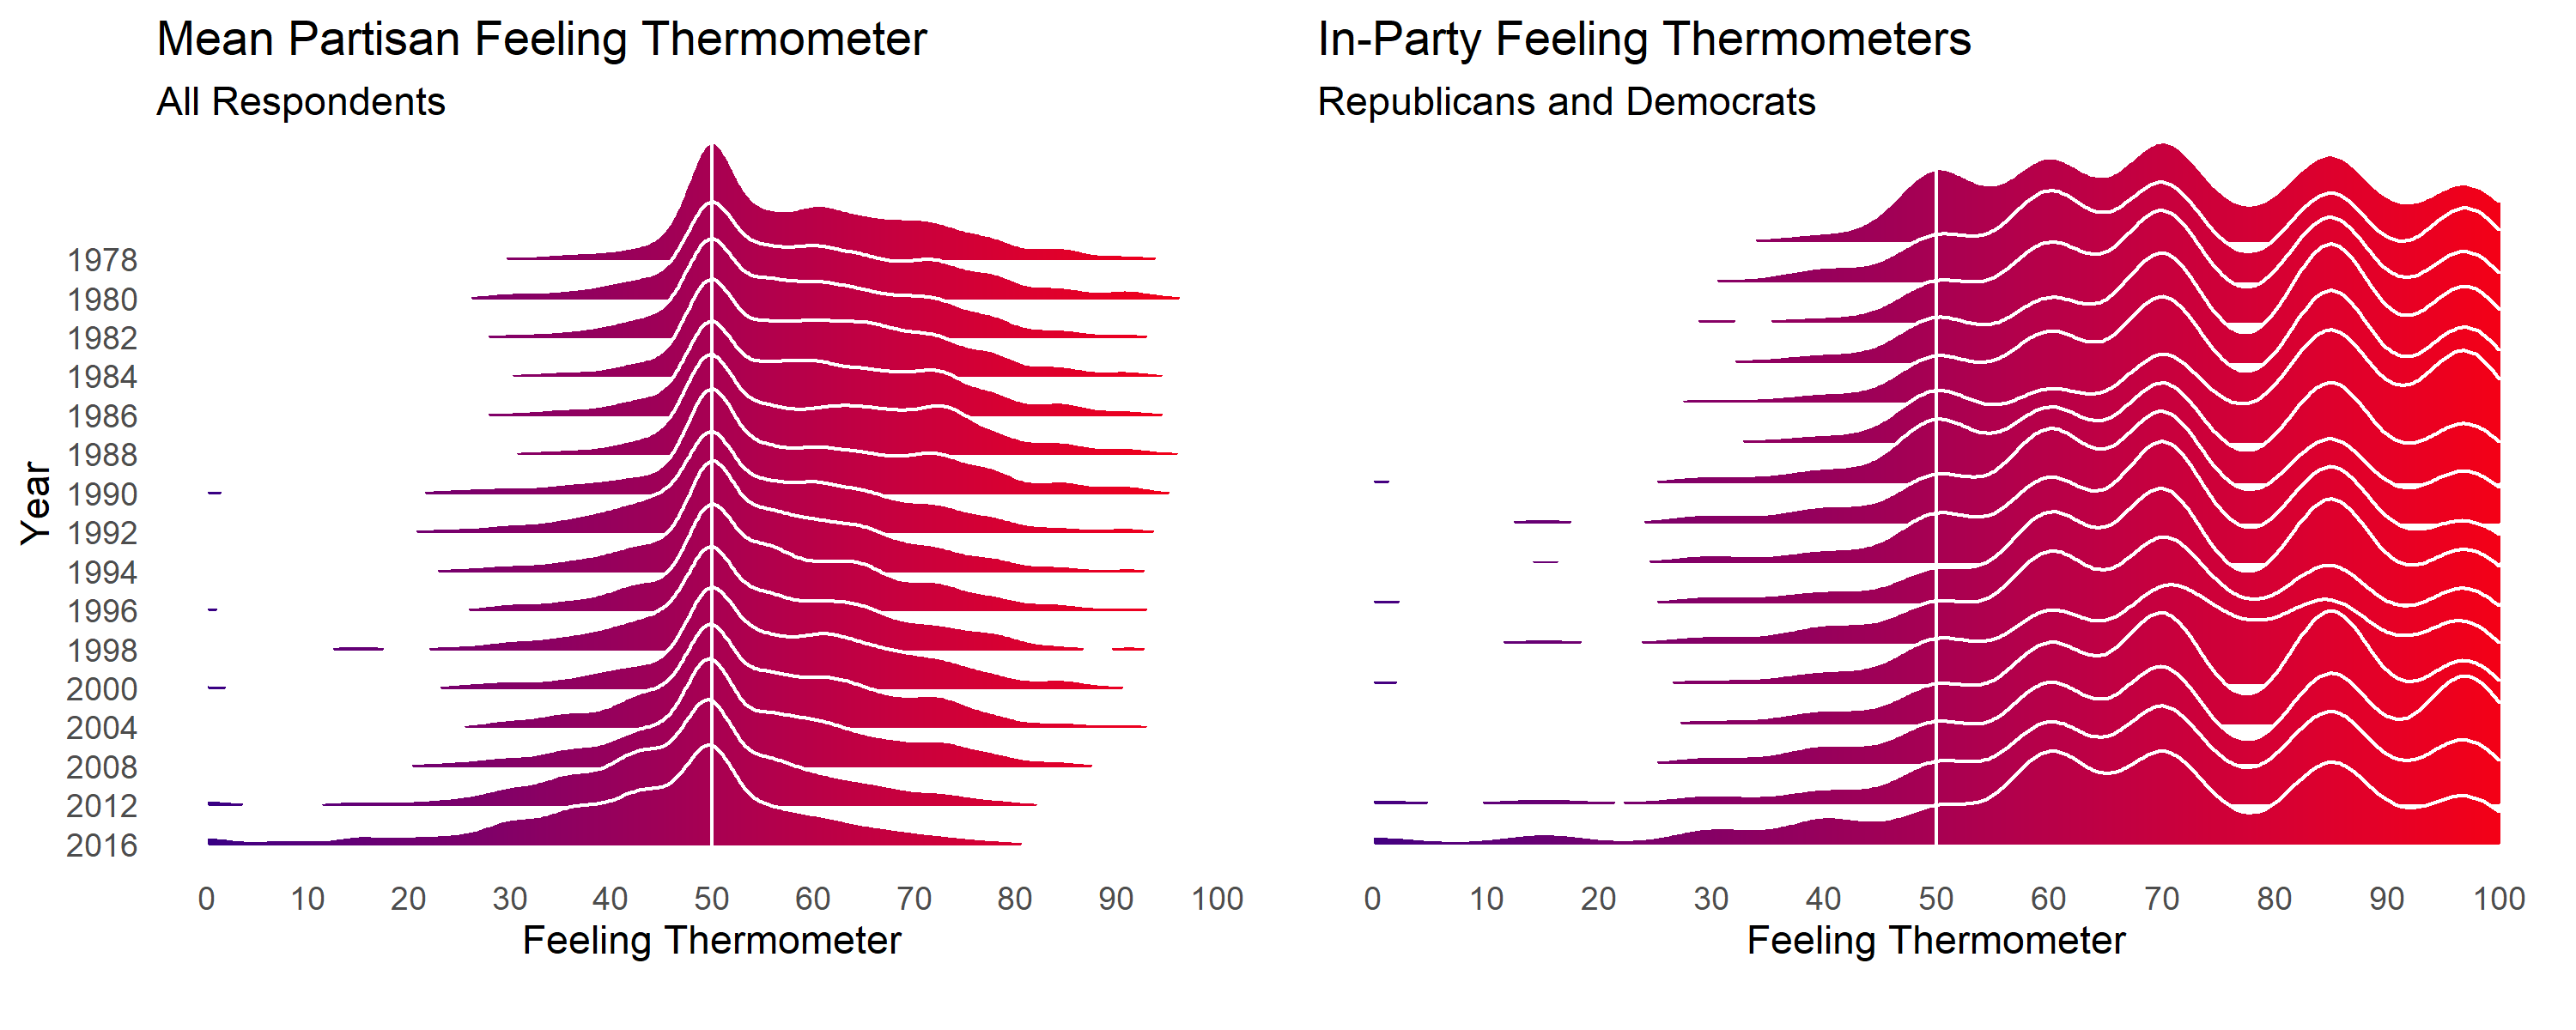
\includegraphics{fig/gg-ridge-grid.png} \emph{\textbf{Fig 4:} These
figures show the changing distribution of partisan affect. The left hand
plot shows the mean partisan FT of Republicans, Democrats, and
Independents. The plot on the right shows only Republican and Democrats'
in-party FT. In both cases, the increasing left skew is apparent.}

Figure 4 shows all respondents' mean partisan feeling thermometer (the
average of their Democrat and Republican thermometers), stratified by
whether the respondent is satisfied or dissatisfied with Democracy.
Unsurprisingly, the leftward tails are largest among discontents, but
all three groups (satisfied, dissatisfied, and those who weren't sure or
declined to answer) have become increasingly likely to be, an average,
cold towards the parties.

\hypertarget{differences-between-cold-and-warm-partisans.}{%
\subsection{Differences Between Cold and Warm
Partisans.}\label{differences-between-cold-and-warm-partisans.}}

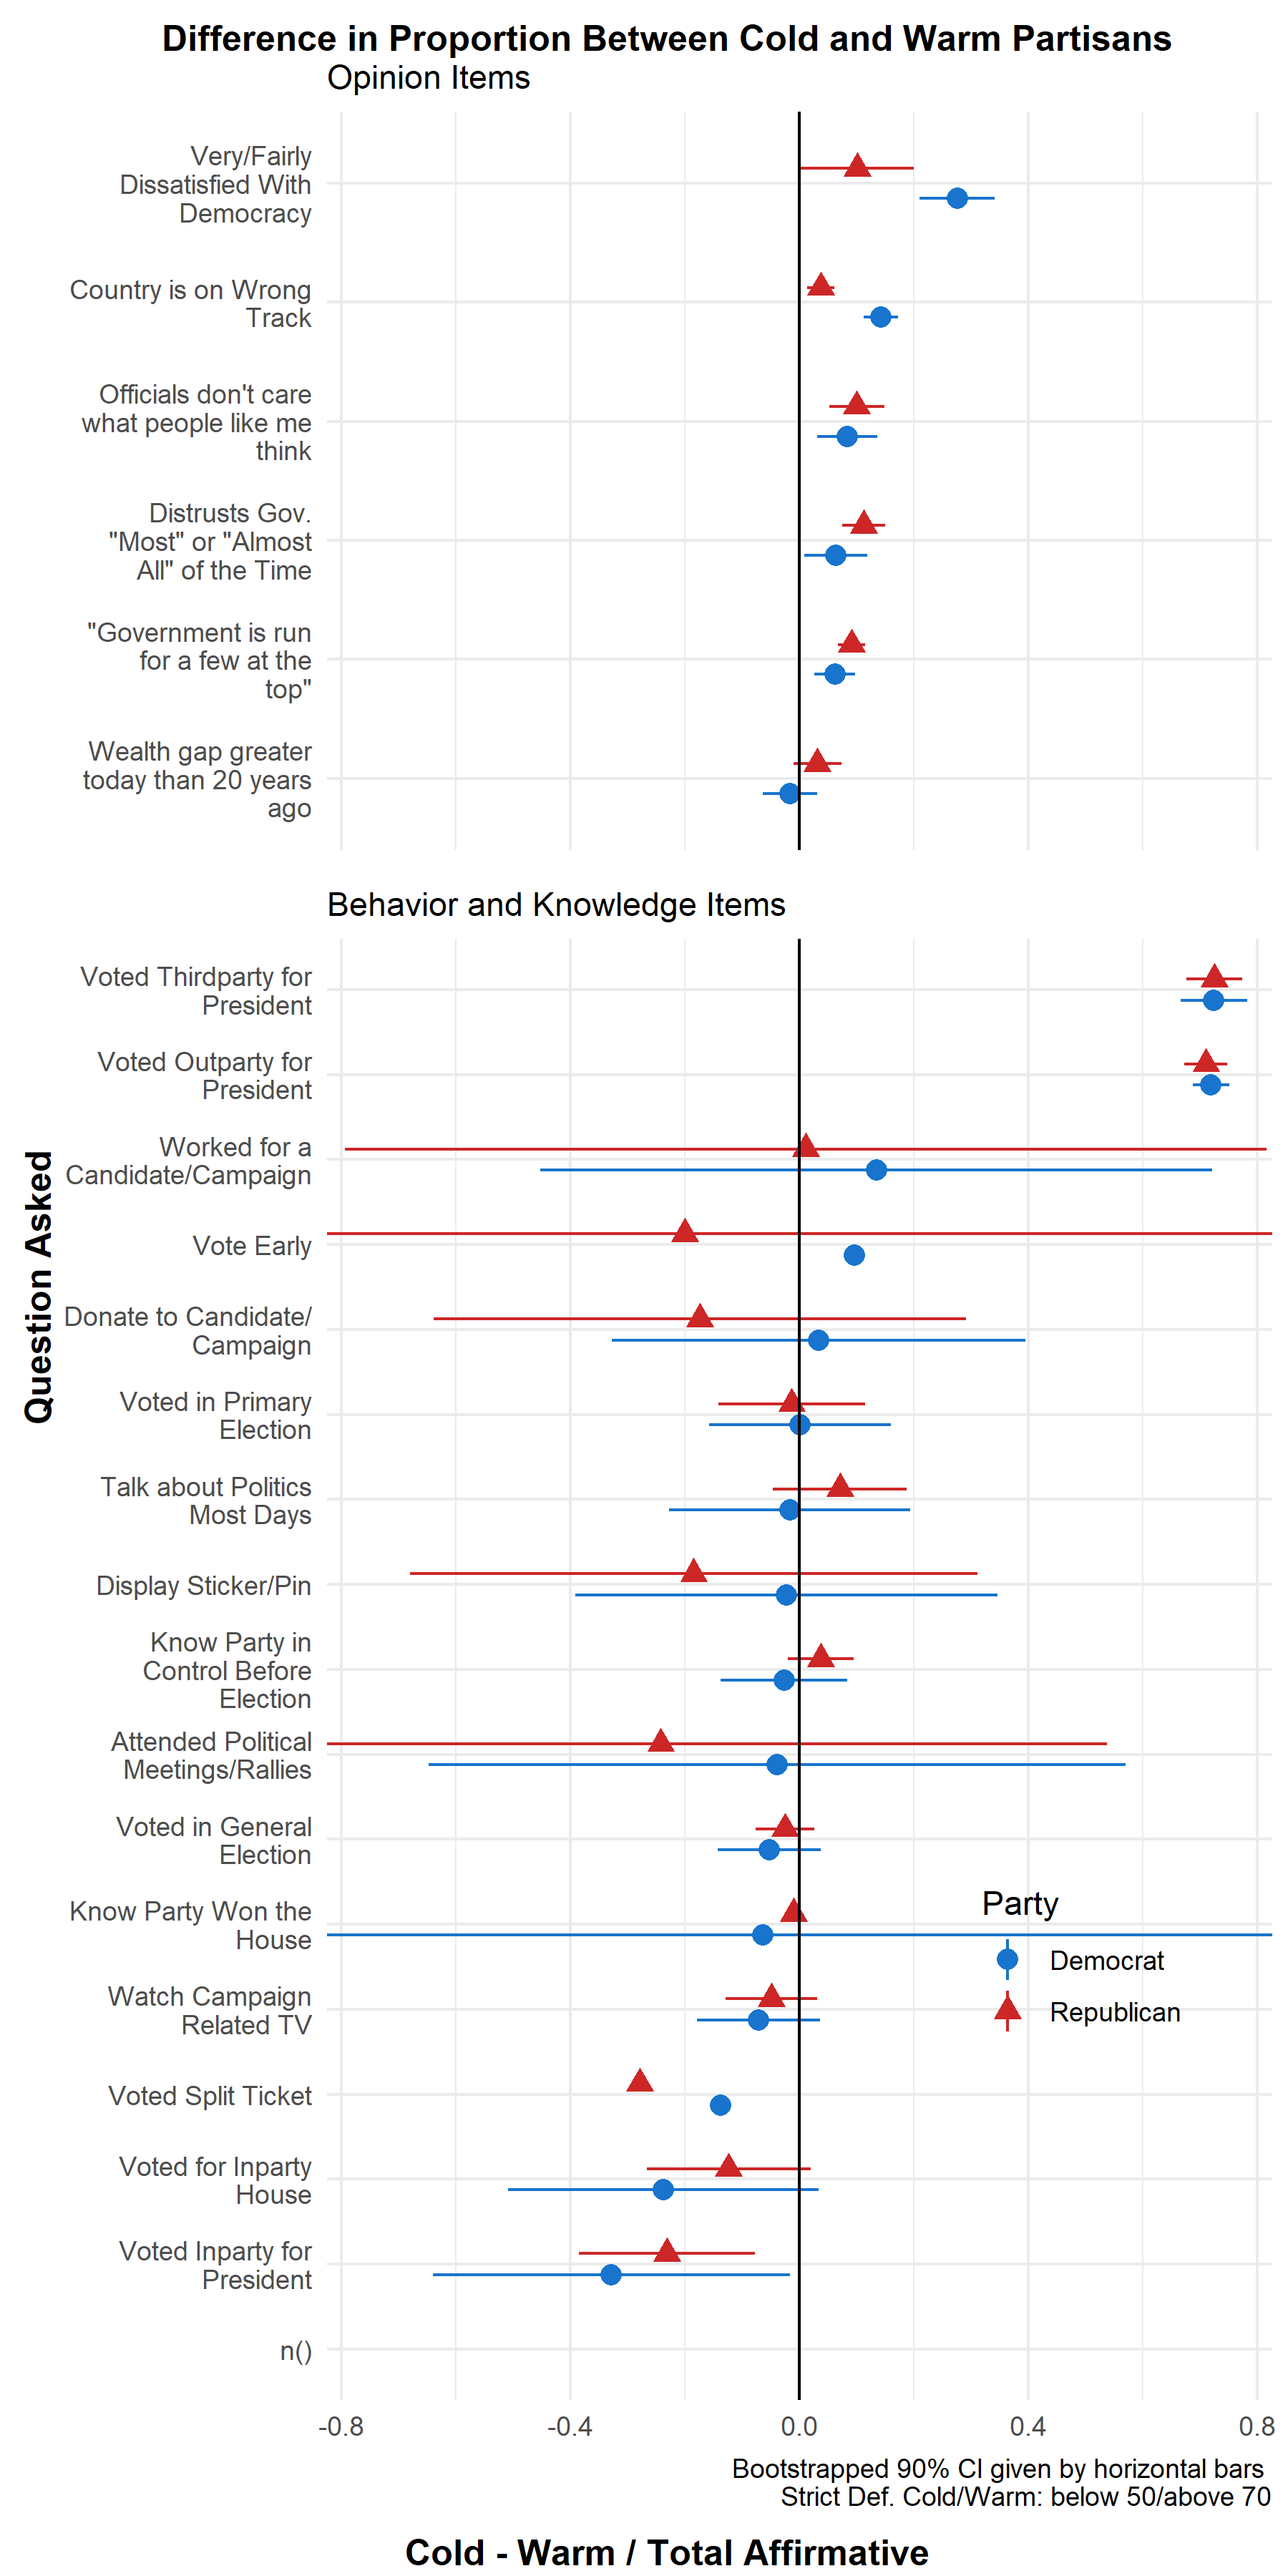
\includegraphics{fig/gg-pooled-combined-strict.png} \emph{\textbf{Fig
5:} Knowledge, opinion, and behavioral differences between cold and warm
partisans. Cold partisans are more pessimistic about government than
their warm co-partisans, and are more likely to support third-party and
major out-party candidates. Interestingly, they are similarly engaged as
their warm counterparts. Voting, campaigning, and discussing politics at
similar rates.}

{[}Add discussion of fig 5, discuss implications of different vote
choices/pessimism{]}

\hypertarget{primaries}{%
\subsection{Primaries}\label{primaries}}

\hypertarget{descriptive-data}{%
\subsubsection{Descriptive Data}\label{descriptive-data}}

I turn now to an examination of the relationship between primary vote
choice and in-party affect. I argue that the increase in cold partisan
affect can be explained in part by ``sore losers'' in primary
elections---as primaries become more salient, so to do the factions
represented by supporters of particular candidates. In short, primary
elections provide another layer of group-based political identity below
the party, forcing partisans to see not just the out-party as
adversarial, but members of their own party as well.

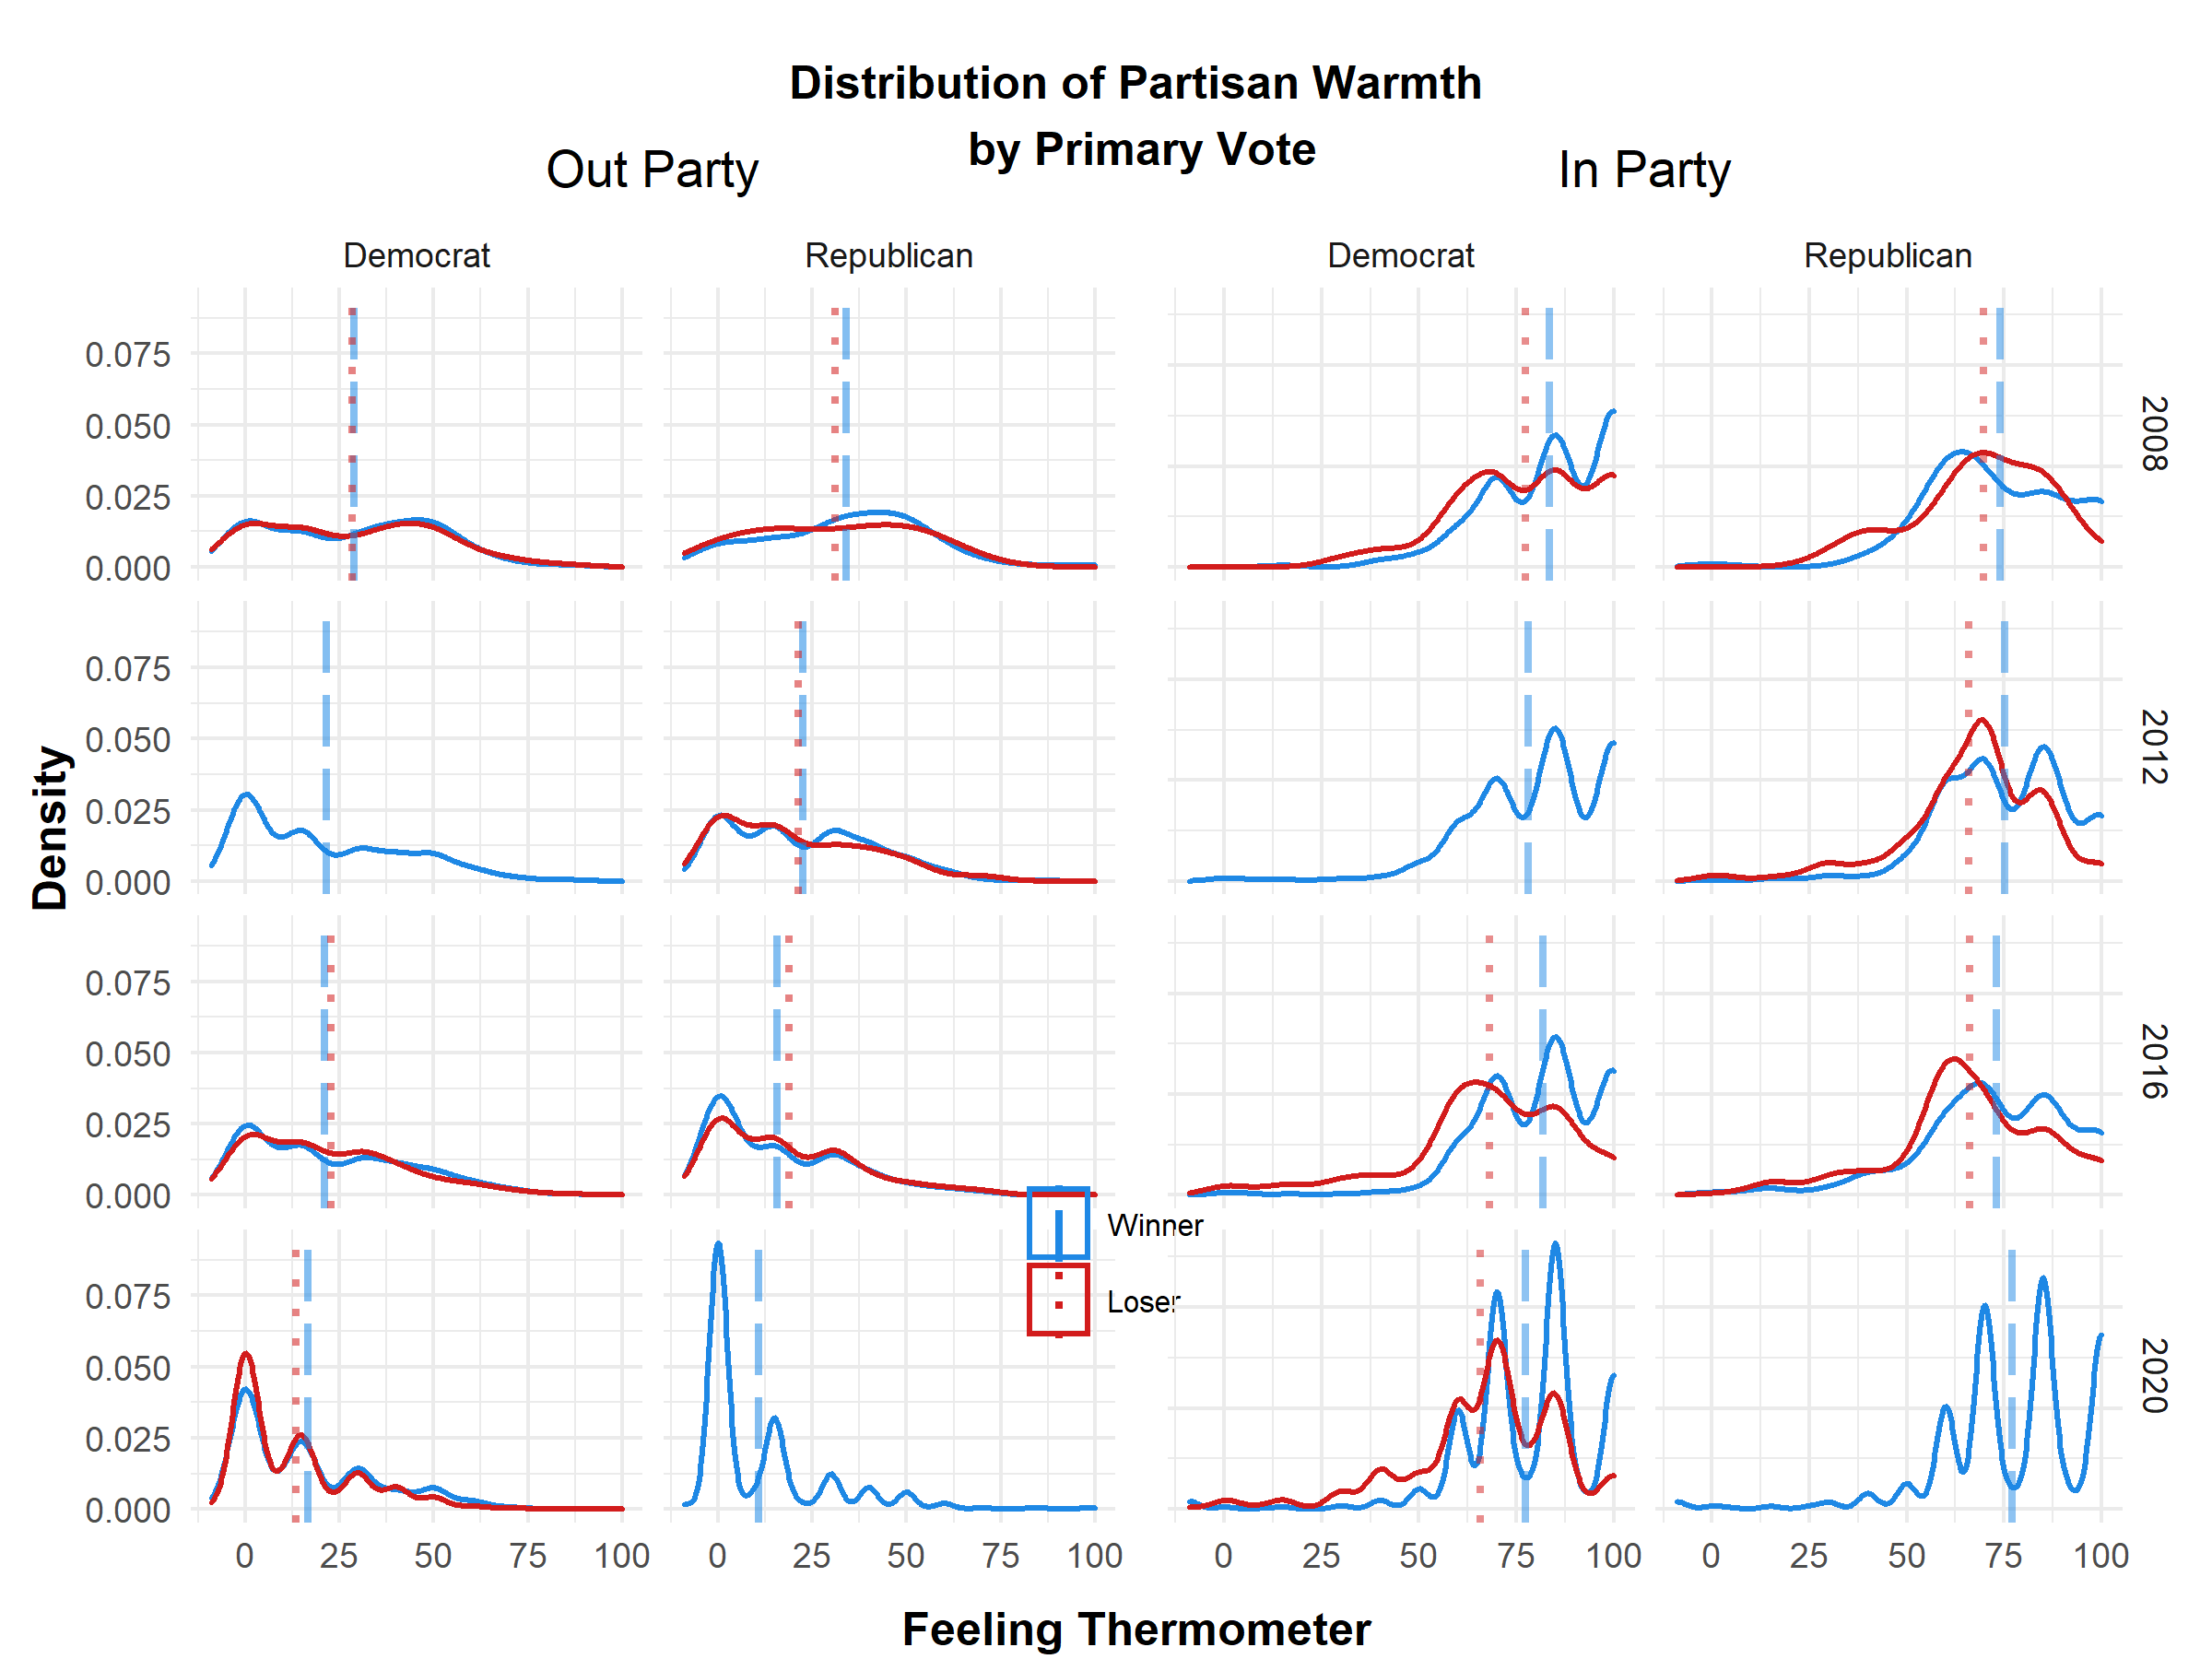
\includegraphics{fig/gg-primaries-grid.png} \emph{\textbf{Fig 6:} Losers
in primaries are colder towards the in-party than winners.} There are
not substantial differences between losers and winners in their
attitudes towards the out-party.*

Primary elections are substantively significant events, allowing
partisans a voice in the presentation and direction of their party. In a
political environment in which the presidential nominee becomes the
\emph{de facto} leader of the party, the primary process affords
non-elite voters a voice in the ideological, political, and stylistic
future of the party. The political products offered by primary
candidates may reflect (or drive) extant divisions in the party.
(Wronski et al. 2018) and (Bankert, n.d.) find that those scoring highly
on measures authoritarian personality traits use their primary vote to
``protect'' their party from factions they see as threatening group
cohesion. Just as voters do not toss a coin to decide their general
election vote, they do not randomly select their choice in the primary;
these choices are likely to be meaningful; if not as matters of
issue-ideology but of political identity.

Figure 6 shows the distribution of in and out-party feeling thermometer
between those who voted for the eventual winners and losers of their
party's primary, as well as those who did not vote.

{[}Expand Section{]}

\hypertarget{panel-data}{%
\subsubsection{Panel Data}\label{panel-data}}

To overcome the problem of observational equivalence inherent to the
cross-sectional ANES, I leverage a series of panel studies conducted by
the National Annenburg Election Survey and the American National
Election Study. Following Lenz (2013), I plan to employ a series of
``three-wave tests'' of the effect of a primary loss on various outcome
variables; strength of partisan identification, general election voting
behavior, political activism, and partisan warmth.

\clearpage

\hypertarget{references}{%
\section*{References}\label{references}}
\addcontentsline{toc}{section}{References}

\hypertarget{refs}{}
\begin{cslreferences}
\leavevmode\hypertarget{ref-bankert2020authoritarian}{}%
Bankert, Alexa. n.d. ``The Authoritarian Divide in the Democratic
Party.'' \emph{Working Paper}.

\leavevmode\hypertarget{ref-clarke2017party}{}%
Clarke, Andrew J. 2017. ``Party Sub-Brands and American Party
Factions.'' \emph{American Journal of Political Science}.

\leavevmode\hypertarget{ref-iyengar2018strengthening}{}%
Iyengar, Shanto, and Masha Krupenkin. 2018. ``The Strengthening of
Partisan Affect.'' \emph{Political Psychology} 39: 201--18.

\leavevmode\hypertarget{ref-iyengar2012affect}{}%
Iyengar, Shanto, Gaurav Sood, and Yphtach Lelkes. 2012. ``Affect, Not
Ideology: A Social Identity Perspective on Polarization.'' \emph{Public
Opinion Quarterly} 76 (3): 405--31.

\leavevmode\hypertarget{ref-klar2016independent}{}%
Klar, Samara, and Yanna Krupnikov. 2016. \emph{Independent Politics}.
Cambridge University Press.

\leavevmode\hypertarget{ref-klar2018affective}{}%
Klar, Samara, Yanna Krupnikov, and John Barry Ryan. 2018. ``Affective
Polarization or Partisan Disdain? Untangling a Dislike for the Opposing
Party from a Dislike of Partisanship.'' \emph{Public Opinion Quarterly}
82 (2): 379--90.

\leavevmode\hypertarget{ref-lenz2013follow}{}%
Lenz, Gabriel S. 2013. \emph{Follow the Leader?: How Voters Respond to
Politicians' Policies and Performance}. University of Chicago Press.

\leavevmode\hypertarget{ref-wronski2018tale}{}%
Wronski, Julie, Alexa Bankert, Karyn Amira, April A Johnson, and Lindsey
C Levitan. 2018. ``A Tale of Two Democrats: How Authoritarianism Divides
the Democratic Party.'' \emph{The Journal of Politics} 80 (4): 1384--8.
\end{cslreferences}

\end{document}
